\documentclass[class=scrbook, crop=false]{standalone}
\usepackage[subpreambles=true]{standalone}
\ifstandalone
    % WARNING: Proceed with caution!

% -----------------------------------------------------------------------------------
% For package standalone
% -----------------------------------------------------------------------------------
\usepackage{import}

% -----------------------------------------------------------------------------------
% Language and typeset
% -----------------------------------------------------------------------------------
\usepackage[ngerman, english]{babel}

\usepackage{subcaption}
% Umlauts and other special characters (UTF-8)
% \usepackage[utf8]{inputenc}
\usepackage{fontspec}
\setsansfont{Arial}
% \usepackage[T1]{fontenc}  % Enable accented characters and umlauts
% LuaLatex doesn't need fontenc and uses UTF-8
% \usepackage{lmodern}  % Font face


% --------------------------------------------------------------------------------
% Page formatting
% --------------------------------------------------------------------------------
% Change the header/footer for chapter beginnings and normal pages
\usepackage[automark,headsepline]{scrlayer-scrpage}

% The package provides an easy and flexible user interface to customize the page
% layout, implementing auto-centering and auto-balancing mechanisms
% WARNING: WHEN CHANGING BCOR (Binding correction), the cover needs reworking!...
\newcommand{\theBCOR}{15mm}  % Define binding correction
\usepackage[
    bindingoffset=\theBCOR,
    % showframe, % Show boxes which indicate margins and paddings
    bottom = 3.5cm, % Margins
      left = 2.5cm,
     right = 2.5cm
] {geometry}

% The package 'float' provides a container for document objects which can not be
% broken over pages, such as tables and figures
% Needed for table and figure indexes  
\usepackage{float}

% support for landscape layout
\usepackage{lscape}

% support of \tablenotes command to add notes under table
\usepackage{threeparttable}

% To allow drawing more professional tables
\usepackage{booktabs}

% --------------------------------------------------------------------------------
% Contents
% --------------------------------------------------------------------------------
% Vector graphics (for Cover page)
\usepackage{tikz} 

% Allows additional parameters when including images
\usepackage{graphicx}

% Roman font family for all headings
\addtokomafont{disposition}{\rmfamily}

% Set the line spacing to 1.5
\usepackage[onehalfspacing]{setspace}

% Improves overall text spacing
% http://www.khirevich.com/latex/microtype/
\usepackage[stretch=10]{microtype}

% Math symbols like mu outside the math environment
\usepackage{textcomp}

% A comprehensive (SI) units package∗
% For defining SI units
\usepackage[
    range-units=single,         % Formatting ranges with single unit indication: 1 - 2 m
    range-phrase=-,             % Phrase for range: 1 - 2 m vs 1 to 2 m
    separate-uncertainty=true,  % sets +- between value and uncertainty 
    multi-part-units=repeat     % In expressions with multiple values (multi part numbers) 
                                % the unit is printed each time: 1 mm x 1 mm
] {siunitx}
% https://tex.stackexchange.com/questions/124488/multi-part-numbers-and-units-in-siunitx

% Allows Sourcecodes with highlighting 
\usepackage{listings}

% This package provides user control over the layout of the three basic list
% environments: enumerate, itemize and description
\usepackage{enumitem}
\setlist{nosep} % Remove the vertical space between \item elements in all lists

% ToDo Notes
% \setlength{\marginparwidth}{2cm}
\usepackage{todonotes}
\setuptodonotes{inline, inlinepar}
\reversemarginpar  % Put ToDo notes on the binding's side
% \usepackage{soul} % Colorful ToDo notes

% Check out colors here http://latexcolor.com/
\usepackage{xcolor}

\usepackage{amsmath}    % alignment of equations

% --------------------------------------------------------------------------------
% Other elements
% --------------------------------------------------------------------------------
% Blindtext: Organic looking text dummy
\usepackage{blindtext}

% Hyperlinks within the document (PDF)
% "hidelinks" hides visual highlighting of links
\usepackage[hidelinks]{hyperref}

% Package for Glossary and Index (Acronyms are listed in a separate list) 
\usepackage[acronym, nogroupskip]{glossaries}[=v4.49] % groupskip: alphabetic grouping of entries

\usepackage{xltabular}   % <------- FOR glossaries

% Integration and management of bibliographies
\usepackage{csquotes}   % backend=biber in biblatex needs this package
\usepackage[
    style=ieee,   % style of the bibliography, entries are sorted in alphabetic order. "ieee" is another common style.
    backend=biber,      % based on package 'biber' 
    bibencoding=ascii   % ASCII Text encoding; may use "utf8" instead
] {biblatex}

% --------------------------------------------------------------------------------
%                               PATHS & FILES
% --------------------------------------------------------------------------------
% Fix paths for standalone compiling
\ifstandalone
    \def \home {..}
\else
    \def \home {.}
\fi

% Package: scrlayer-scrpage
% \def \stylePath {\home/settings+/style/page}
\input{\home/settings+/style/page}  % Load page style

% Package: graphicx
\graphicspath{{\home/images/}}  % Set path to images

% Package: listings
\input{\home/settings+/style/code.tex}  % Set path to style file
\lstset{inputpath={\home/code/}} % Default path to code listings

% Package: glossaries
\input{\home/settings+/style/symbols}  % Set path to symbols list style file
\input{\home/settings+/style/acronyms}  % Set path to acronym list style file
% -------------------------------------------------------------------------------
%               Listing of all Glossary and Acronym Entries 
%                           use as shown below
% -------------------------------------------------------------------------------

% ==== EXEMPLARY ENTRY FOR SYMBOLS LIST =========================================

% ==== EXEMPLARY ENTRY FOR ACRONYMS LIST ========================================
% \newacronym{#label}{#acronym}{#long_form}

% define new command for custom arconym entry with only two arguments
% fabricates an easier way to use \newacronym 
\newcommand{\acroX}[2]{\newacronym{#1}{#1}{#2}}
% \acroX{label and arconym}{long name}
% \acroX{CD}               {Compact Disk}

\newcommand{\acroY}[3]{\newacronym{#1}{#2}{#3}}
% \arcoY{label}{acronym}{long name}
% \acroY{CD}   {cd}     {Compact Disk}
 
\newacronym{AEP}{AEP}{Imbalance price}
\newacronym{aFRR}{aFRR}{Automatic Frequency Restoration Reserve}


\newacronym{reBAP}{reBAP}{Uniform imbalance price}
\newacronym{TSO}{TSO}{Transmission System Operator}
\newacronym{FCR}{FCR}{Frequency Containment Reserve}
\newacronym{mFRR}{mFRR}{Manual Frequency Restoration Reserve}
\newacronym{BRP}{BRP}{Balancing Responsible Party}
\newacronym{SB}{SB}{System Balance}
\newacronym{VRE}{VRE}{variable renewable energy}
\newacronym{ID1}{ID1}{intraday index ID1}
\newacronym{MAE}{MAE}{mean average error}
\newacronym{RMSE}{RMSE}{root mean squared error}
\newacronym{MSE}{MSE}{mean squared error}
\newacronym{CRPS}{CRPS}{continuous ranked probabililty score}
\newacronym{GCC}{GCC}{Grid Control Cooperation}
\newacronym{IC}{IC}{Continuous intraday}
\newacronym{VWAP}{VWAP}{volume-weighted average price}
\newacronym{VID}{VID}{traded volume within the intraday market}
\newacronym{ID AEP}{ID AEP}{Intraday Average Energy Price}
\newacronym{FRR}{FRR}{Frequency Restoration Reserve}
\newacronym{TFT}{TFT}{Temporal Fusion Transformer}
\newacronym{DLM}{DLM}{Dynamic Linear Model}
\newacronym{GB}{GB}{Gradient Boosting}
\newacronym{RF}{RF}{Random Forest}
\newacronym{ARIMAX}{ARIMAX}{Autoregressive Integrated Moving Average with eXogenous variables}
\newacronym{xLSTM}{xLSTM}{Extended Long Short-Term Memory}
\newacronym{DWD}{DWD}{Deutscher Wetterdienst}
\newacronym{ENTSO-E}{ENTSO-E}{European Network of Transmission System Operators for Electricity}
\newacronym{IDA1}{IDA1}{Intraday auction 1}
\newacronym{MOSMIX}{MOSMIX}{Model Output Statistics-MIX}
\newacronym{mLSTM}{mLSTM}{memory-optimized LSTM}
\newacronym{sLSTM}{sLSTM}{speed-optimized LSTM}

% ==== EXEMPLARY ENTRY FOR MAIN GLOSSARY ========================================

    % \newglossaryentry{policy}{name={Policy},description={Im geschäftlichen Bereich bezeichnet Policy eine interne Leit- bzw. Richtlinie, die formal durch das Unternehmen dokumentiert und über ihr Management verantwortet wird}}
    % \newglossaryentry{pcie}{name={PCI Express},description={PCI Express („Peripheral Component Interconnect Express“, abgekürzt PCIe oder PCI-E) ist ein Standard zur Verbindung von Peripheriegeräten mit dem Chipsatz eines Hauptprozessors. PCIe ist der Nachfolger von PCI, PCI-X und AGP und bietet im Vergleich zu seinen Vorgängern eine höhere Datenübertragungsrate pro Pin.}}
    % \newglossaryentry{realnumber}
  % Load glossary, symbol and acronyms list

% Package: biblatex
\addbibresource{\home/references/references.bib}  % Set path to bib resources

% Custom variables
\input{\home/settings+/variables}
% --------------------------------------------------------------------------------
%                                   OPTIONAL
% --------------------------------------------------------------------------------


% Simple arithmetic for LaTeX commands
% \usepackage{calc}

% Document Elements
% -------------------

% Index
% \usepackage{imakeidx}

% compact Lists
%\usepackage{paralist}

% visual improvements for citations
% \usepackage{epigraph}

% Create pseudo code
% https://www.overleaf.com/learn/latex/Algorithms
% \usepackage{algorithm}
% \usepackage{algorithmic}
%\usepackage[noend]{algpseudocode}

% Formatting
% -------------------
% Tweaks for scrbook, redefines commands of other packages
% \usepackage{scrhack}

% Intelligent space separator (nice for superscript?)
% \usepackage{xspace}

% Allows breaks within tables
%\usepackage{tabularx}

% Allows for page breaks in tables
% \usepackage{longtable}

% allows modifying of captions
% \usepackage{caption}

% Multiline comments
%\usepackage{verbatim}

% % Custom colors
% \definecolor{dartmouthgreen}{rgb}{0.05, 0.5, 0.06}

% IF you want to define unicode characters
% \DeclareUnicodeCharacter{0229}{\c{e}}
% \DeclareUnicodeCharacter{0306}{\u{Z}}


% Document elements
% ------------------------------------

% Table package
% \usepackage{booktabs}

% Pie diagram
% \usepackage{datapie}

% Side by Side images
% \usepackage{subcaption}

% For landscape tables
%\usepackage{pdflscape}
%\usepackage{afterpage}

% Graphics can be flow around by text
%\usepackage{wrapfig}

\fi

% ----------------------------------------------------------------------------
%                               Theoretical Background
% ----------------------------------------------------------------------------
\begin{document}

%\ifstandalone
   % \selectlanguage{ngerman}  % Toggle ON/OFF

    % Language-specific settings that change automatically
    %\input{settings+/language}
%\fi

\chapter{Theoretical Background}
\label{Chapter::Theoretical_Background} % Outline text
This chapter provides background knowledge to understand the concepts in the thesis.

% Background topics that are necessary to understand your thesis
\section{German electricity market}
\label{Section::German_Electricity_Market}

In the German electricity market, each market participant is referred to as a \gls{BRP}. \gls{BRP}s are responsible for submitting energy schedules to the \gls{TSO}s that reflect their expected electricity generation and consumption.
Their goal is to keep their portfolio balanced, meaning that scheduled generation aligns with expected consumption.

Both generation and consumption are subject to uncertainty and can deviate from the submitted schedules. On the generation side, this is particularly relevant for \gls{VRE} sources such as wind and solar, whose output depends heavily on weather conditions. Similarly, energy consumption varies with social patterns—for instance, workdays versus weekends, or regular days versus school holidays \cite{neumannUsingWeatherData2023} \cite{el-azabSeasonalForecastingHourly2025}. 

Based on historical data and forecasts, \gls{BRP}s create schedules that are submitted to the \gls{TSO}s ahead of time. However due to forecast errors or sudden changes in weather or consumption, the physically delivered volumes may deviate from the submitted schedules \cite{InvestigationSystemImbalances}. In such cases, the \gls{BRP}’s portfolio is considered imbalanced. 

The deviations of all \gls{BRP}s within a balancing area are aggregated to calculate the \gls{SB} of that area. Across all German balancing areas, these are combined to form the \gls{GCC} balance. The  \gls{GCC} balance indicates whether the system, as a whole, is short or long on energy.

To maintain a stable grid frequency of 50 Hz, \gls{TSO}s must deploy balancing energy in response to the current system balance. If there is a shortage of energy (positive imbalance), \gls{TSO}s activate positive balancing energy—either by ramping up partially loaded generators or reducing demand via controllable loads. If the system has a surplus of  energy (negative imbalance), negative balancing energy is deployed—this may involve ramping down generators or increasing load (e.g., by activating flexible consumers) \cite{ActivatingReserves}. 

The imbalance volumes and associated prices are then calculated by the \gls{TSO}s and passed on to the  \gls{BRP}s.  \gls{BRP}s whose portfolios contributed to the system imbalance—e.g., being short when the system is also short—must pay the imbalance price for the volume in question. Conversely, \gls{BRP}s who help stabilize the system—e.g., by having a surplus when the system is short—are compensated accordingly. 

Understanding this market structure, including the balancing responsibilities and the mechanisms used by  \gls{TSO}s, is essential for modeling and predicting the  \gls{reBAP}. Section \ref{Section::Imbalance_Price} provides a detailed explanation of how this price is determined in detail. 

%This energy can be positive, if the grid is short of energy, or negative, if the grid has a surplus of energy. 

%If the system is in need of energy, reserve generators that run below full capacity can be activated to increase their production. Another way of introducing positive balancing energy into the grid is turning off variable loads to decrease energy consumption.

%If the system has a surplus of energy, negative balancing energy has to be dispatched. This can be done either by throttleing capacity generators which are running above minimum capacity. Negative balancing energy can also be inserted into the grid by turning on variable loads, leading to an increased energy consumption.

%The imbalance price is calculated and forwarded onto the BRPs. 
%How this price is calculated will be explained in the next chapter.%
%Each BRP whose portfolio led to increasing the system balance, for example having provided not enough energy whilst the system is also short of energy, has to pay the imbalance price for the volume of their imbalance. 
%On the other hand, BRPs which helped stabilize the system with their portfolio, for example providing more energy than consumed while the system is short of energy, are remunerated for their imbalance. 
%Next, the different auctions and their schedule will be explained. An overview can be found in \ref{fig::energy_auctions}. 

\begin{figure}[ht]
            \centering
            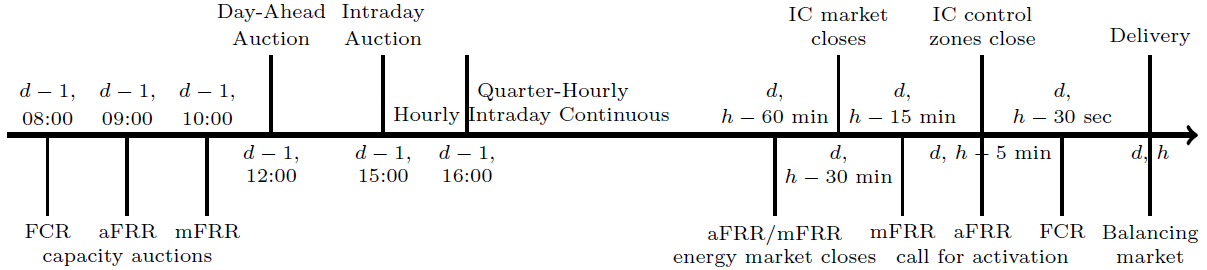
\includegraphics[width=\textwidth]{theory/energy_auctions.png}
            \caption[Timeschedule for energy market auctions]{Timeline of market auctions, intraday trading, and balancing energy activation leading up to delivery. Times are shown relative to delivery day 
d and hour 
h \cite{narajewskiProbabilisticForecastingGerman2022}.}
            \label{fig::energy_auctions}
 \end{figure}

Figure \ref{fig::energy_auctions} illustrates the auction and balancing sequence of the German electricity market, relative to the delivery timestamp (d, h).
The timeline begins on the previous day with three reserve capacity auctions:  \gls{FCR} at 08:00, aFRR at 09:00, and  \gls{mFRR} at 10:00. These auctions determine the prices for positive and negative balancing reserves, but since no data was available during this thesis, they are excluded from the analysis \cite{narajewskiProbabilisticForecastingGerman2022} .

The Day-Ahead auction follows at 12:00, and the Intraday Auction is held at 15:00.  \gls{IC} trading opens at 16:00 and continues until shortly before delivery. Unlike discrete auction events, \gls{IC} allows trading on a rolling basis \cite{EPEXTradingBrochure} \cite{narajewskiProbabilisticForecastingGerman2022} \cite{EPEXTradingBrochure}.

The \gls{IC} market closes in stages: cross-zone trades close 30 minutes before delivery, while trades within a single control zone remain possible until 5 minutes before delivery. This timestamp — 5 minutes before physical delivery — is referred to as the gate closure time throughout this thesis \cite{narajewskiProbabilisticForecastingGerman2022}  \cite{EPEXTradingBrochure}.

Understanding this market timing is essential, as it determines which information is available at prediction time, and directly influences both \gls{BRP} behavior and the imbalance price formation.

 
 
%On the far right of the figure the time of delivery is shown, denoted by $d$, $h$ of the delivery. The auctions for this timestamp start the day before. From $8:00$ to $10:00$ on the previous day reserve capacity auctions take place. These auctions decide the price for positive and negative balancing energy.
%Data about these auctions was not available at the time of this thesis, so no information about these auctions will be used throughout this thesis.
%The first auction takes place at $12:00$ one day before delivey and is called the day ahead (DA) auction. At $15:00$ the next auction, the intraday auction (IA) takes place. After that, at $16:00$ intraday continuous trading (IC) starts. Whilst the auctions are a single auction event, during the intraday continuous (IC) trading window energy can be traded at any time. The IC has different closing times. Up until $30$ minutes before delivery energy can be traded across all control zones. Trades on IC that happen within a single control zone can be done up until $5$ minutes before delivery.

%For the rest of the thesis the timestamp $5$ mintues before delivery time will be called the gate closure time.

%\subsection{Terminology}

%\subsubsection{Residual load}

%Residual load is the load  that has to be covered by not variable renewable energey (VRE) sources.
%It can be calculted by substracting the power produced by solar and wind (both off- and onshore) from the total load.

\section{Imbalance price}
\label{Section::Imbalance_Price}

 \begin{figure}[b]
            \centering
            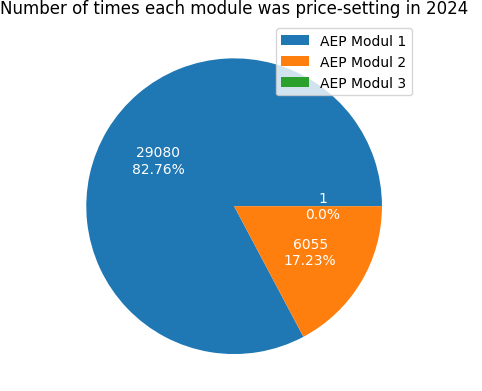
\includegraphics[width=.5\textwidth]{theory/aep_modules.pdf}
             \caption[How often each module was price-setting in 2024?]{How often each module was price-setting in 2024 \cite{NetztransparenzAEPModul}}
            \label{fig::aep_modules}
 \end{figure}
The German imbalance price — also referred to as the \gls{reBAP} — reflects the cost of balancing energy that \gls{BRP}s must pay or receive when their portfolio deviates from the submitted schedule.
To ensure consistency across control zones, a uniform price is calculated for all of Germany. The calculation is based on a modular approach defined by the \gls{TSO}s and regulatory framework \cite{NetztransparenzReBAPDefinition}.

The final imbalance price is determined from the results of three separate modules, each of which reflects a different aspect of the cost and incentive structure:
\begin{itemize}
\item Module 1: The cost of activated balancing reserves
\item Module 2: A market-based incentive to encourage portfolio balancing
\item Module 3: A scarcity signal in extreme imbalance situations
\end{itemize}
The module with the highest financial impact (depending on the sign of the system imbalance) is selected to define the \gls{reBAP} for each 15-minute settlement period. Figure \ref{fig::aep_modules} shows how often each module was price setting in 2024. Module 1 was price setting in 82,76\% and module 2 in 17,23\% of all quarter-hours\cite{NetztransparenzAEPModul}.



\subsection{Module 1: Basis component}
The basis component reflects the actual cost of activating balancing reserves. It serves as the default pricing module and is used in most settlement periods.
Two types of balancing reserves are considered:
\begin{itemize}
\item \gls{aFRR} 
\item \gls{mFRR} 
\end{itemize}

For each reserve, the \gls{VWAP} is calculated using data from the European platforms PICASSO (for \gls{aFRR}) and MARI (for \gls{mFRR}).
This results in four prices for each 15-minute interval:
\begin{itemize}
\item $VWAP_{aFRR}$ (positive and negative)
\item $VWAP_{mFRR}$ (positive and negative)
\end{itemize}

Depending on which reserve was activated, the system calculates the corresponding price ($AEP_1$). If both \gls{aFRR} and \gls{mFRR} were activated, a volume-weighted average of their \gls{VWAP}s is used.
If neither was activated, the avoided activation price is applied, typically computed as the average of the cheapest.

The resulting AEP₁ (either positive or negative) is selected based on the sign of the system balance (GCC balance)\cite{NetztransparenzReBAP}:
\begin{itemize}
\item If the system is short: the positive $AEP_1$ is used
\item If the system is long: the negative $AEP_1$ is used
\item If the system is balanced: the component is set to 0
\end{itemize}
%This module reflects the marginal cost of balancing and forms the foundation of the imbalance price in over 80\% of all intervals.




%The first module is called the basis component. 
%This module represents the cost of providing the balancing energy.

%With information provided by PICASSO the volume-weighted average price for the automatic frequency restoration reserve $VWAP_{aFRR}$ can be calculated. This is calculated for both positive and negative activations, resulting in $VWAP_{aFRR, GCC, pos, qh}$ and $VWAP_{aFRR,  GCC, neg, qh}$ for each quarter hour $qh$ and the GCC balance.
%The same calculations are done for mFRR activations using data from MARI, resulting int $VWAP_{mFRR, GCC, pos, qh}$ and $VWAP_{mFRR, GCC, neg, qh}$. 
%These valuese are used in the formulas \ref{fig::aep1_pos} and \ref{fig::aep1_neg} to calculate the values $AEP1_{pos}$ and $AEP1_{neg}$. 
%If neither aFRR or mFRR were activated during the associated quarter hour this $AEP1$ takes the value of avoided activation. This value is equal to the mean of the cheapest aFRR bid prices for the quarter hour.
%If only one of the reserves was activated $AEP1$ takes the value of the $VWAP$ of that reserve. 
%If both reserves were activated, the $AEP1$ is equal to the volume-weighted average of both $VWAPs$. The volume is denoted by the satisfied demand $SD$.

%\begin{figure}[ht]
%            \centering
%            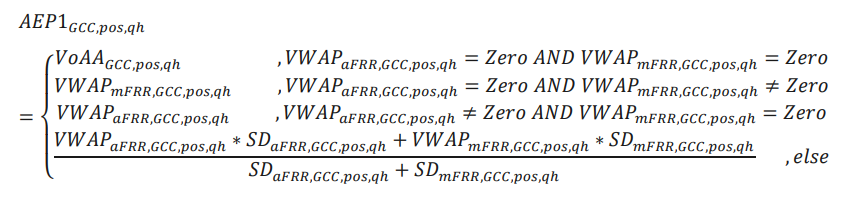
\includegraphics[width=\textwidth]{theory/aep1_pos.png}
%            \caption[Positive AEP 1 component formula]{Positive AEP 1 component formula %\cite{NetztransparenzReBAP}.}
%            \label{fig::aep1_pos}
% \end{figure}
 
 

% \begin{figure}[ht]
%            \centering
%            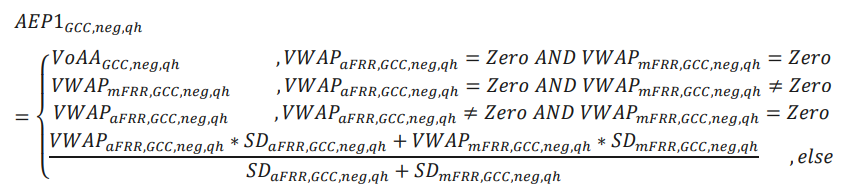
\includegraphics[width=\textwidth]{theory/aep1_neg.png}
%             \caption[Positive AEP 1 component formula]{Positive AEP 1 component formula %\cite{NetztransparenzReBAP}.}
%            \label{fig::aep1_neg}
% \end{figure}

%With both $AEP1s$, the value of the basis component can be calculated. If the system balance is positive, this module takes the value of $AEP1_{GCC, pos, qh}$. If the system balance is negative, this module takes the value of $AEP1_{GCC, neg, qh}$. If the system balance is equal to 0, this module's value is 0.

\subsection{Module 2: Incentivising component}
\label{Section::Module_2}
The incentivising component aims to discourage market participants from relying on imbalance energy and instead motivate them to actively balance their portfolios via intraday trading. The underlying idea is that imbalance energy should be more expensive than purchasing electricity directly on the market — especially shortly before delivery \cite{kochPASSIVEBALANCINGINTRADAY2020a} .

This module is applied only when there is sufficient liquidity in the intraday market for the quarter-hour in question. Specifically, the module is activated if the \gls{VID} for that interval exceeds 500 MW. If this threshold is not reached, the module is skipped, and its value is set to zero.

When activated, the \gls{ID AEP} serves as the reference point for calculating the \gls{reBAP}. This price is computed as the volume-weighted average of the most recent trades summing up to 500 MW (i.e., 125 MWh for a 15-minute period), executed as close as possible to the gate closure time.

To increase the incentive for \gls{BRP}s to remain balanced, the imbalance price is artificially adjusted by introducing a minimum price distance ($\Delta P$) between the \gls{reBAP} and the \gls{ID AEP}. This distance ramps up linearly with the absolute value of the \gls{GCC} system imbalance, up to a maximum value of 25\% of the \gls{ID AEP} — or at least €10/MWh, whichever is higher.

The logic can be summarized as follows:
\begin{itemize}
\item If the system is short (positive GCC balance):
 reBAP = ID AEP + $\Delta P$
\item If the system is long (negative GCC balance):
 reBAP = ID AEP − $\Delta P$
\item If the system is balanced:
 reBAP = ID AEP
\end{itemize}

$\Delta P$ is defined as a linear function of the GCC balance between 0 and ±500 MW. This relationship is visualized in Figure \ref{fig::delta_p_graph}, using a fixed ID AEP of €100/MWh as an example. 

From a forecasting perspective, Module 2 introduces a dynamic, nonlinear pricing logic. 
Since the final price is not directly based on \gls{ID AEP} alone, but also on the size and direction of the system imbalance, accurate forecasts of both \gls{GCC} balance and market prices are essential for reliable reBAP prediction during periods where this module is active.

In 2024, the incentivising component was the price-setting mechanism in 17.23\% of all 15-minute settlement intervals (Figure \ref{fig::aep_modules}). 
%These typically correspond to periods with moderate but directional imbalances, in which active trading signals are available near gate closure.

The next section discusses Module 3, which is triggered under conditions of extreme imbalance and scarcity of reserves.

%The goal behind module 2 is to increase the reBAP, so that it is more costly to use imbalance energy than buying the need energy on the intraday market. This should incentivise all BRPs to keep their portfolio balanced. 
%The formula for its calculation is displayed in figure \ref{fig::aep2}.and will be explained in the next paragraphs.

%For each settlement period $V_{ID}$ denotes the volume of total trades that were closed on the intraday market for this quarter. If this volume is below $500$MW, this component finds no application and takes the value of 0. If value was greater than $500$MW this module is calculated using the Intraday Price Index (ID AEP) and a minimum distance $\Delta P$. 
%The ID AEP is calculated for each quarter hour by averaging over the trades closest to the delivery time. For this calculation only a volume of 500 MW, so 125 MW/h for a quarter hour is considered.  
%The volume-weighted average price is formed from the transactions filtered this way. 
%In the case that the GCC balance is equal to 0, this module takes the value of ID AEP.  In the case of a positive GCC balance, a minimum distance $\Delta P$ is added onto the ID AEP, in case of a negative GCC balance this $\Delta P$ is substracted from the ID AEP. Between ID AEP and module 2 a minimum distance of $25\%$, but at least 10€ is established, assuming the absolute value of the GCC balance is equal to or greater than $500$ MW. This distance $\Delta P$ linearly ramps up from $0$MW to $500$MW. The formula for $\Delta P$ can be found in figure \ref{fig::delta_p} and a graph for its values with a fixed ID AEP of $100€/MWh$ is displayed in figure \ref{fig::delta_p_graph}.


 \begin{figure}[ht]
            \centering
            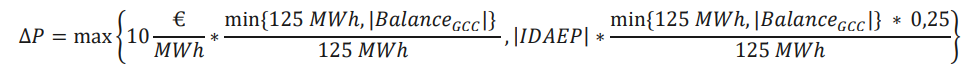
\includegraphics[width=.7\textwidth]{theory/delta_p.pdf}
             \caption[Graph for $\Delta P$ with a fixed ID AEP for $100€/MWh$]{Graph for $\Delta P$ with a fixed ID AEP for $100€/MWh$.}
            \label{fig::delta_p_graph}
 \end{figure}

 %\begin{figure}[ht]
%            \centering
%            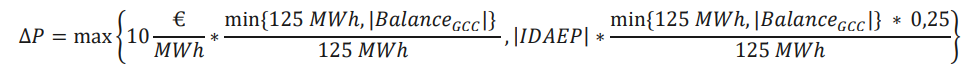
\includegraphics[width=\textwidth]{theory/delta_p.png}
%             \caption[Formula for$ \Delta P$]{Formula for $\Delta P$ .}
%            \label{fig::delta_p}
% \end{figure}
%  \begin{figure}[ht]
%            \centering
%            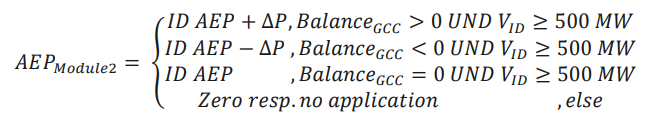
\includegraphics[width=\textwidth]{theory/aep_2.png}
%             \caption[Formula for $AEP_{Module 2}$]{Formula for $AEP_{Module 2}$.}
%            \label{fig::aep2}
% \end{figure}

\subsection{Module 3: Scarcity component}

%If the GCC balance exceeds $80\%$ of the frequency restoration reserve (FRR) for a settlement period, the scarcity component is applied. This component rarely is the price setting module of the reBAP (<1\%). The formula for this module will not be discussed here. Figure \ref{fig::aep_3} shows a graph of how this module's value changes relatively to the GCC balance.


% \begin{figure}[ht]
 %           \centering
  %          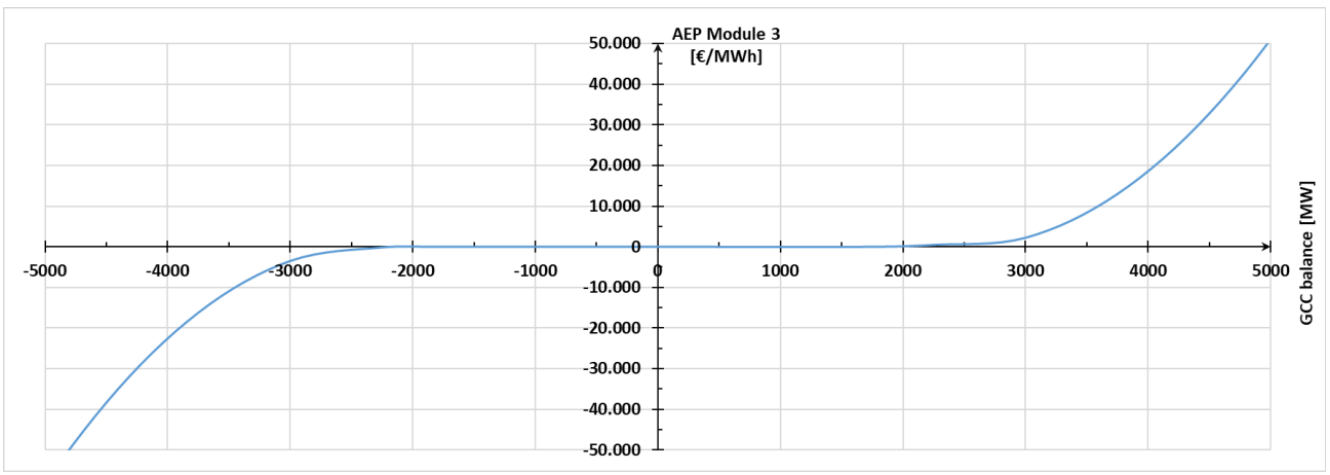
\includegraphics[width=\textwidth]{theory/aep_3.png}
%             \caption[Graph how the price of module 3 correlates with GCC balance]{Graph how the price of module 3 %correlates with GCC balance .}
%            \label{fig::aep_3}
% \end{figure}

The scarcity component is designed to reflect critical system conditions in which balancing reserves are nearly exhausted. It serves as an economic signal to incentivize all market participants to avoid any further deviation from their schedules under extreme imbalance situations.

This module is only activated if the \gls{GCC} balance (i.e., the aggregated system imbalance across all German control areas) exceeds 80\% of the available \gls{FRR} in a given settlement period. This threshold marks a high-stress scenario in which the grid approaches its technical limits for balancing energy provision.

When triggered, the scarcity component applies a penalty mechanism that leads to significantly higher imbalance prices compared to the other modules. However, due to its strict activation criteria, the module is rarely used in practice. In the year 2024, the scarcity component was the price-setting module in only one quarter-hour 

The exact formula for Module 3 is not discussed here, as its impact on overall \gls{reBAP} behavior is negligible from a statistical perspective. 
To provide an estimate of the values this module can take: in the one instance where Module 3 was price-setting in 2024, its value amounted to $10.097/MWh€$. 

Depending on the sign of the imbalance, the \gls{reBAP} is set to:
\begin{itemize}
\item the maximum of the three module values if the system is short (positive \gls{GCC} balance), or
\item the minimum if the system is long (negative \gls{GCC} balance)
\end{itemize}

This selection logic is applied uniformly across all modules. Figure \ref{fig::aep_modules} summarizes the percentage of intervals in 2024 in which each module determined the reBAP.
Even though Module 3 rarely sets the price, its existence serves as a critical backstop in the regulatory design — signaling the potential for extreme system stress and providing strong economic disincentives for imbalance during those periods.

%Depeding on the sign of the GCC balance, either the minimum or the maximum of the three modules introduced in the previous paragraphs is used. The formula for this is displayed in figure \ref{fig::rebap_neg}. If the GCC balance is positive, the module with the highest value is used. If the balance is negative the cheapest module is used to determine the reBAP.

%For the whole year 2024 the reBAP was equal to the basis component $82.76\%$, equal to the incentivising component $17.23\%$ and equal to the scarcity component $0.00\%$ of the time, with the scarcity component only being the price setting module once throughout 2024. This data is displayed in figure \ref{fig::aep_modules}.




% You can use this to add content for standalone documents if you like
% In this case we would like to show the references.
\ifstandalone
    % Bibliography
    \printbibliography[heading=bibintoc]                         \cleardoublepage

% ----------------------------------------------------------------------------
% Appendix and Glossary
% ----------------------------------------------------------------------------
%     \pagenumbering{Alph} % A, B, C..

% %     % Appendix
%     \documentclass[class=scrbook, crop=false]{standalone}
\usepackage[subpreambles=true]{standalone}
\ifstandalone
    % WARNING: Proceed with caution!

% -----------------------------------------------------------------------------------
% For package standalone
% -----------------------------------------------------------------------------------
\usepackage{import}

% -----------------------------------------------------------------------------------
% Language and typeset
% -----------------------------------------------------------------------------------
\usepackage[ngerman, english]{babel}

\usepackage{subcaption}
% Umlauts and other special characters (UTF-8)
% \usepackage[utf8]{inputenc}
\usepackage{fontspec}
\setsansfont{Arial}
% \usepackage[T1]{fontenc}  % Enable accented characters and umlauts
% LuaLatex doesn't need fontenc and uses UTF-8
% \usepackage{lmodern}  % Font face


% --------------------------------------------------------------------------------
% Page formatting
% --------------------------------------------------------------------------------
% Change the header/footer for chapter beginnings and normal pages
\usepackage[automark,headsepline]{scrlayer-scrpage}

% The package provides an easy and flexible user interface to customize the page
% layout, implementing auto-centering and auto-balancing mechanisms
% WARNING: WHEN CHANGING BCOR (Binding correction), the cover needs reworking!...
\newcommand{\theBCOR}{15mm}  % Define binding correction
\usepackage[
    bindingoffset=\theBCOR,
    % showframe, % Show boxes which indicate margins and paddings
    bottom = 3.5cm, % Margins
      left = 2.5cm,
     right = 2.5cm
] {geometry}

% The package 'float' provides a container for document objects which can not be
% broken over pages, such as tables and figures
% Needed for table and figure indexes  
\usepackage{float}

% support for landscape layout
\usepackage{lscape}

% support of \tablenotes command to add notes under table
\usepackage{threeparttable}

% To allow drawing more professional tables
\usepackage{booktabs}

% --------------------------------------------------------------------------------
% Contents
% --------------------------------------------------------------------------------
% Vector graphics (for Cover page)
\usepackage{tikz} 

% Allows additional parameters when including images
\usepackage{graphicx}

% Roman font family for all headings
\addtokomafont{disposition}{\rmfamily}

% Set the line spacing to 1.5
\usepackage[onehalfspacing]{setspace}

% Improves overall text spacing
% http://www.khirevich.com/latex/microtype/
\usepackage[stretch=10]{microtype}

% Math symbols like mu outside the math environment
\usepackage{textcomp}

% A comprehensive (SI) units package∗
% For defining SI units
\usepackage[
    range-units=single,         % Formatting ranges with single unit indication: 1 - 2 m
    range-phrase=-,             % Phrase for range: 1 - 2 m vs 1 to 2 m
    separate-uncertainty=true,  % sets +- between value and uncertainty 
    multi-part-units=repeat     % In expressions with multiple values (multi part numbers) 
                                % the unit is printed each time: 1 mm x 1 mm
] {siunitx}
% https://tex.stackexchange.com/questions/124488/multi-part-numbers-and-units-in-siunitx

% Allows Sourcecodes with highlighting 
\usepackage{listings}

% This package provides user control over the layout of the three basic list
% environments: enumerate, itemize and description
\usepackage{enumitem}
\setlist{nosep} % Remove the vertical space between \item elements in all lists

% ToDo Notes
% \setlength{\marginparwidth}{2cm}
\usepackage{todonotes}
\setuptodonotes{inline, inlinepar}
\reversemarginpar  % Put ToDo notes on the binding's side
% \usepackage{soul} % Colorful ToDo notes

% Check out colors here http://latexcolor.com/
\usepackage{xcolor}

\usepackage{amsmath}    % alignment of equations

% --------------------------------------------------------------------------------
% Other elements
% --------------------------------------------------------------------------------
% Blindtext: Organic looking text dummy
\usepackage{blindtext}

% Hyperlinks within the document (PDF)
% "hidelinks" hides visual highlighting of links
\usepackage[hidelinks]{hyperref}

% Package for Glossary and Index (Acronyms are listed in a separate list) 
\usepackage[acronym, nogroupskip]{glossaries}[=v4.49] % groupskip: alphabetic grouping of entries

\usepackage{xltabular}   % <------- FOR glossaries

% Integration and management of bibliographies
\usepackage{csquotes}   % backend=biber in biblatex needs this package
\usepackage[
    style=ieee,   % style of the bibliography, entries are sorted in alphabetic order. "ieee" is another common style.
    backend=biber,      % based on package 'biber' 
    bibencoding=ascii   % ASCII Text encoding; may use "utf8" instead
] {biblatex}

% --------------------------------------------------------------------------------
%                               PATHS & FILES
% --------------------------------------------------------------------------------
% Fix paths for standalone compiling
\ifstandalone
    \def \home {..}
\else
    \def \home {.}
\fi

% Package: scrlayer-scrpage
% \def \stylePath {\home/settings+/style/page}
\input{\home/settings+/style/page}  % Load page style

% Package: graphicx
\graphicspath{{\home/images/}}  % Set path to images

% Package: listings
\input{\home/settings+/style/code.tex}  % Set path to style file
\lstset{inputpath={\home/code/}} % Default path to code listings

% Package: glossaries
\input{\home/settings+/style/symbols}  % Set path to symbols list style file
\input{\home/settings+/style/acronyms}  % Set path to acronym list style file
% -------------------------------------------------------------------------------
%               Listing of all Glossary and Acronym Entries 
%                           use as shown below
% -------------------------------------------------------------------------------

% ==== EXEMPLARY ENTRY FOR SYMBOLS LIST =========================================

% ==== EXEMPLARY ENTRY FOR ACRONYMS LIST ========================================
% \newacronym{#label}{#acronym}{#long_form}

% define new command for custom arconym entry with only two arguments
% fabricates an easier way to use \newacronym 
\newcommand{\acroX}[2]{\newacronym{#1}{#1}{#2}}
% \acroX{label and arconym}{long name}
% \acroX{CD}               {Compact Disk}

\newcommand{\acroY}[3]{\newacronym{#1}{#2}{#3}}
% \arcoY{label}{acronym}{long name}
% \acroY{CD}   {cd}     {Compact Disk}
 
\newacronym{AEP}{AEP}{Imbalance price}
\newacronym{aFRR}{aFRR}{Automatic Frequency Restoration Reserve}


\newacronym{reBAP}{reBAP}{Uniform imbalance price}
\newacronym{TSO}{TSO}{Transmission System Operator}
\newacronym{FCR}{FCR}{Frequency Containment Reserve}
\newacronym{mFRR}{mFRR}{Manual Frequency Restoration Reserve}
\newacronym{BRP}{BRP}{Balancing Responsible Party}
\newacronym{SB}{SB}{System Balance}
\newacronym{VRE}{VRE}{variable renewable energy}
\newacronym{ID1}{ID1}{intraday index ID1}
\newacronym{MAE}{MAE}{mean average error}
\newacronym{RMSE}{RMSE}{root mean squared error}
\newacronym{MSE}{MSE}{mean squared error}
\newacronym{CRPS}{CRPS}{continuous ranked probabililty score}
\newacronym{GCC}{GCC}{Grid Control Cooperation}
\newacronym{IC}{IC}{Continuous intraday}
\newacronym{VWAP}{VWAP}{volume-weighted average price}
\newacronym{VID}{VID}{traded volume within the intraday market}
\newacronym{ID AEP}{ID AEP}{Intraday Average Energy Price}
\newacronym{FRR}{FRR}{Frequency Restoration Reserve}
\newacronym{TFT}{TFT}{Temporal Fusion Transformer}
\newacronym{DLM}{DLM}{Dynamic Linear Model}
\newacronym{GB}{GB}{Gradient Boosting}
\newacronym{RF}{RF}{Random Forest}
\newacronym{ARIMAX}{ARIMAX}{Autoregressive Integrated Moving Average with eXogenous variables}
\newacronym{xLSTM}{xLSTM}{Extended Long Short-Term Memory}
\newacronym{DWD}{DWD}{Deutscher Wetterdienst}
\newacronym{ENTSO-E}{ENTSO-E}{European Network of Transmission System Operators for Electricity}
\newacronym{IDA1}{IDA1}{Intraday auction 1}
\newacronym{MOSMIX}{MOSMIX}{Model Output Statistics-MIX}
\newacronym{mLSTM}{mLSTM}{memory-optimized LSTM}
\newacronym{sLSTM}{sLSTM}{speed-optimized LSTM}

% ==== EXEMPLARY ENTRY FOR MAIN GLOSSARY ========================================

    % \newglossaryentry{policy}{name={Policy},description={Im geschäftlichen Bereich bezeichnet Policy eine interne Leit- bzw. Richtlinie, die formal durch das Unternehmen dokumentiert und über ihr Management verantwortet wird}}
    % \newglossaryentry{pcie}{name={PCI Express},description={PCI Express („Peripheral Component Interconnect Express“, abgekürzt PCIe oder PCI-E) ist ein Standard zur Verbindung von Peripheriegeräten mit dem Chipsatz eines Hauptprozessors. PCIe ist der Nachfolger von PCI, PCI-X und AGP und bietet im Vergleich zu seinen Vorgängern eine höhere Datenübertragungsrate pro Pin.}}
    % \newglossaryentry{realnumber}
  % Load glossary, symbol and acronyms list

% Package: biblatex
\addbibresource{\home/references/references.bib}  % Set path to bib resources

% Custom variables
\input{\home/settings+/variables}
% --------------------------------------------------------------------------------
%                                   OPTIONAL
% --------------------------------------------------------------------------------


% Simple arithmetic for LaTeX commands
% \usepackage{calc}

% Document Elements
% -------------------

% Index
% \usepackage{imakeidx}

% compact Lists
%\usepackage{paralist}

% visual improvements for citations
% \usepackage{epigraph}

% Create pseudo code
% https://www.overleaf.com/learn/latex/Algorithms
% \usepackage{algorithm}
% \usepackage{algorithmic}
%\usepackage[noend]{algpseudocode}

% Formatting
% -------------------
% Tweaks for scrbook, redefines commands of other packages
% \usepackage{scrhack}

% Intelligent space separator (nice for superscript?)
% \usepackage{xspace}

% Allows breaks within tables
%\usepackage{tabularx}

% Allows for page breaks in tables
% \usepackage{longtable}

% allows modifying of captions
% \usepackage{caption}

% Multiline comments
%\usepackage{verbatim}

% % Custom colors
% \definecolor{dartmouthgreen}{rgb}{0.05, 0.5, 0.06}

% IF you want to define unicode characters
% \DeclareUnicodeCharacter{0229}{\c{e}}
% \DeclareUnicodeCharacter{0306}{\u{Z}}


% Document elements
% ------------------------------------

% Table package
% \usepackage{booktabs}

% Pie diagram
% \usepackage{datapie}

% Side by Side images
% \usepackage{subcaption}

% For landscape tables
%\usepackage{pdflscape}
%\usepackage{afterpage}

% Graphics can be flow around by text
%\usepackage{wrapfig}

\fi

% ----------------------------------------------------------------------------
%                                 Appendix
% ----------------------------------------------------------------------------
\begin{document}
\appendix

\chapter{}
\addcontentsline{toc}{chapter}{Some Appendix}
\label{Chapter::Some Appendix}
Stuff that was not important or too much for the thesis but is still important or complements the presented results.

\section{Section A}
\label{Section::Some Appendix:Section A}


\begin{table}[]
\begin{tabular}{l|l}
Parameter & Description \\\hline
 ABSF\_STD & Hourly value for absolute humidity \\
   D & Wind direction\\
   F & Wind speed\\
   FF & Wind speed (10 minute average)\\
 FX\_911	& Fastest gust of wind in the last hour \\
   P	& Air pressure at NN \\
   P0	 & Air pressure at Station \\
   P\_STD & Hourly value for air pressure \\
   R1 & Hourly precipitation height \\
   RF\_STD	& Hourly value for relative humidity \\
   RF\_TU & Relative humidity \\
   RS\_IND	& Precipitation indicator (yes/no) \\
   SD\_SO	 & Hourly sunshine duration \\
   TD	 & Dew point temperature \\
   TD\_STD	& Dew point temperature in 2m height\\
   TF\_STD & Hourly value for humidity temperature\\
   TT	 & Temperature in 2m height \\
   TT\_TU & Air temperature \\
   V\_N & Cloud coverage (all clouds) \\
   V\_S1\_CS	 & Cloud type (first layer) \\
   V\_S1\_CSA & Cloud type abbreviation (first layer) \\
   V\_S1\_HHS	& Cloud height (first layer) \\
   V\_S1\_NS	 & Cloud coverage (first layer) \\
   V\_S2\_CS & Cloud type (second layer) \\
   V\_S2\_CSA & Cloud type abbreviation (second layer) \\
   V\_S2\_HHS	& Cloud height (second layer) \\
   V\_S2\_NS	 & Cloud coverage (second layer) \\
   V\_S3\_CS & Cloud type (third layer) \\
   V\_S3\_CSA & Cloud type abbreviation (third layer) \\
   V\_S3\_HHS	& Cloud height (third layer) \\
   V\_S3\_NS	 & Cloud coverage (third layer) \\
   V\_S4\_CS & Cloud type (fourth layer) \\
   V\_S4\_CSA & Cloud type abbreviation (fourth layer) \\
   V\_S4\_HHS	& Cloud height (fourth layer) \\
   V\_S4\_NS	 & Cloud coverage (fourth layer) \\
   V\_VV	& Visibility\\
  
   WRTR & Hourly Precipitaion form \\
   WW & Hourly observed weather \\ 
   
\end{tabular}
\caption{Variables in DWD measurement data}
\label{Table::DWD_Measurement_Parameters}
\end{table}


\begin{table}[]
\begin{tabular}{l|l}
Parameter & Description \\\hline
DD & Wind direction\\
FF & Wind speed\\
FX1 & Maximum wind gust within the last hour\\
FX3 & Maximum wind gust within the last 3 hours\\
FXh & Maximum wind gust within the last 12 hours\\
FXh25 & Probability of wind gusts >= 25kn within the last 12 hours\\
FXh40 & Probability of wind gusts >= 40kn within the last 12 hours\\
FXh55 & Probability of wind gusts >= 55kn within the last 12 hours\\
N & Total cloud cover\\
N05 & Cloud cover below 500 ft.\\
Neff & Effective cloud cover\\
Nh & High cloud cover (>7 km)\\
Nl & Low cloud cover (lower than 2 km)\\
Nm & Midlevel cloud cover (2-7 km)\\
PPPP & Surface pressure, reduced\\
R602 & Probability of precipitation > 0.2mm during the last 6 hours\\
R650 & Probability of precipitation > 5.0mm during the last 6 hours\\
RR1c & Total precipitation during the last hour consistent with significant weather\\
RR3c & Total precipitation during the last 3 hours consistent with significant weather\\
RRS1c & Snow-Rain-Equivalent during the last hour\\
RRS3c & Snow-Rain-Equivalent during the last 3 hours\\
Rad1h & Global Irradiance\\
Rd02 & Probability of precipitation > 0.2mm during the last 24 hours\\
Rd50 & Probability of precipitation > 5.0mm during the last 24 hours\\
Rh00 & Probability of precipitation > 0.0mm during the last 12 hours\\
Rh02 & Probability of precipitation > 0.2mm during the last 12 hours\\
Rh10 & Probability of precipitation > 1.0mm during the last 12 hours\\
Rh50 & Probability of precipitation > 5.0mm during the last 12 hours\\
SunD1 & Sunshine duration during the last Hour\\
T5cm & Temperature 5cm above surface\\
TN & Minimum temperature - within the last 12 hours\\
TTT & Temperature 2m above surface\\
TX & Maximum temperature - within the last 12 hours\\
Td & Dewpoint 2m above surface\\
VV & Visibility\\
W1W2 & Past weather during the last 6 hours\\
ww & Significant Weather\\
wwM & Probability for fog within the last hour\\
wwM6 & Probability for fog within the last 6 hours\\
wwMh & Probability for fog within the last 12 hours\\
\end{tabular}
\caption{Variables in DWD MOSMIX data}
\label{Table::DWD_MOSMIX_Parameters}
\end{table}

\subsection{Subsection B}
\label{Subsection::Some Appendix:Subsection B}

\Blindtext
\chapter{}
\addcontentsline{toc}{chapter}{Some Appendix2}

\blindtext
\Blindtext

\end{document}
                                          \clearpage

% %     % Symbol list also counts as a glossary object
%     \printglossary[type=main]  % main glossary

% %     % Either print all entries or only used entries for all lists
%     \glsaddallunused
\fi

\end{document}
